\subsection{Impedancia de entrada}
Para medir la impedancia de entrada del circuito en funci\'on de la frecuencia, 
deb\'iamos hacer el cociente $V_{in}/I_{in}$. Si bien se puede medir la tensi\'on 
de entrada al circuito de forma directa con el osciloscopio, 
no es tan sensillo obtener la corriente que entra al circuito, ya que el osciloscopio 
mide tensiones y no corrientes. Se busc\'o una resistencia $R_L$ cuyo valor comerical 
fuera lo m\'as parecido posible (igual o el primero mayor) al valor obtenido en 
el c\'alculo te\'rico para cada uno de los casos de resistencias. Se coloc\'o dicha 
resistencia en serie al generador, a la entrada del circuito. Luego se midi\'o la ca\'ida 
de tensi\'on sobre ella, ya que al dividirla por el valor de la $R_L$ colocada se obtendr\'ia 
la corriente de entrada al circuito $I_{in}$. El criterio de buscar una resistencia similar 
al valor calculado de $Z_{in}$ surge de que si se pusiese una resistencia muy chica, 
la diferencia entre las tensiones medidas sobre sus bornes ser\'ia muy chica 
(aumentando incertidumbre) y si se colocase una resistencia muy grande, 
la tensi\'on que caer\'ia ser\'ia mucho mayor a la que caer\'ia en el circuito, 
haciendo que la tensi\'on luego de la resistencia sea muy chica (se podr\'ia 
acercar al nivel de ruido) y que la diferencia de tensi\'on entre sus bornes tienda 
a la tensi\'on entregada por el generador. Por eso se consider\'o \'optimo que la 
resistencia tenga un valor similar al calculado de forma te\'orica y en caso de no 
conseguir el mismo valor, prefiri\'endose un valor mayor y no menor. 


En los siguientes gr\'aficos se observa la impedancia de entrada medida y simulada con el m\'etodo de Montecarlo.
\begin{figure}[H] %!ht
	\centering
	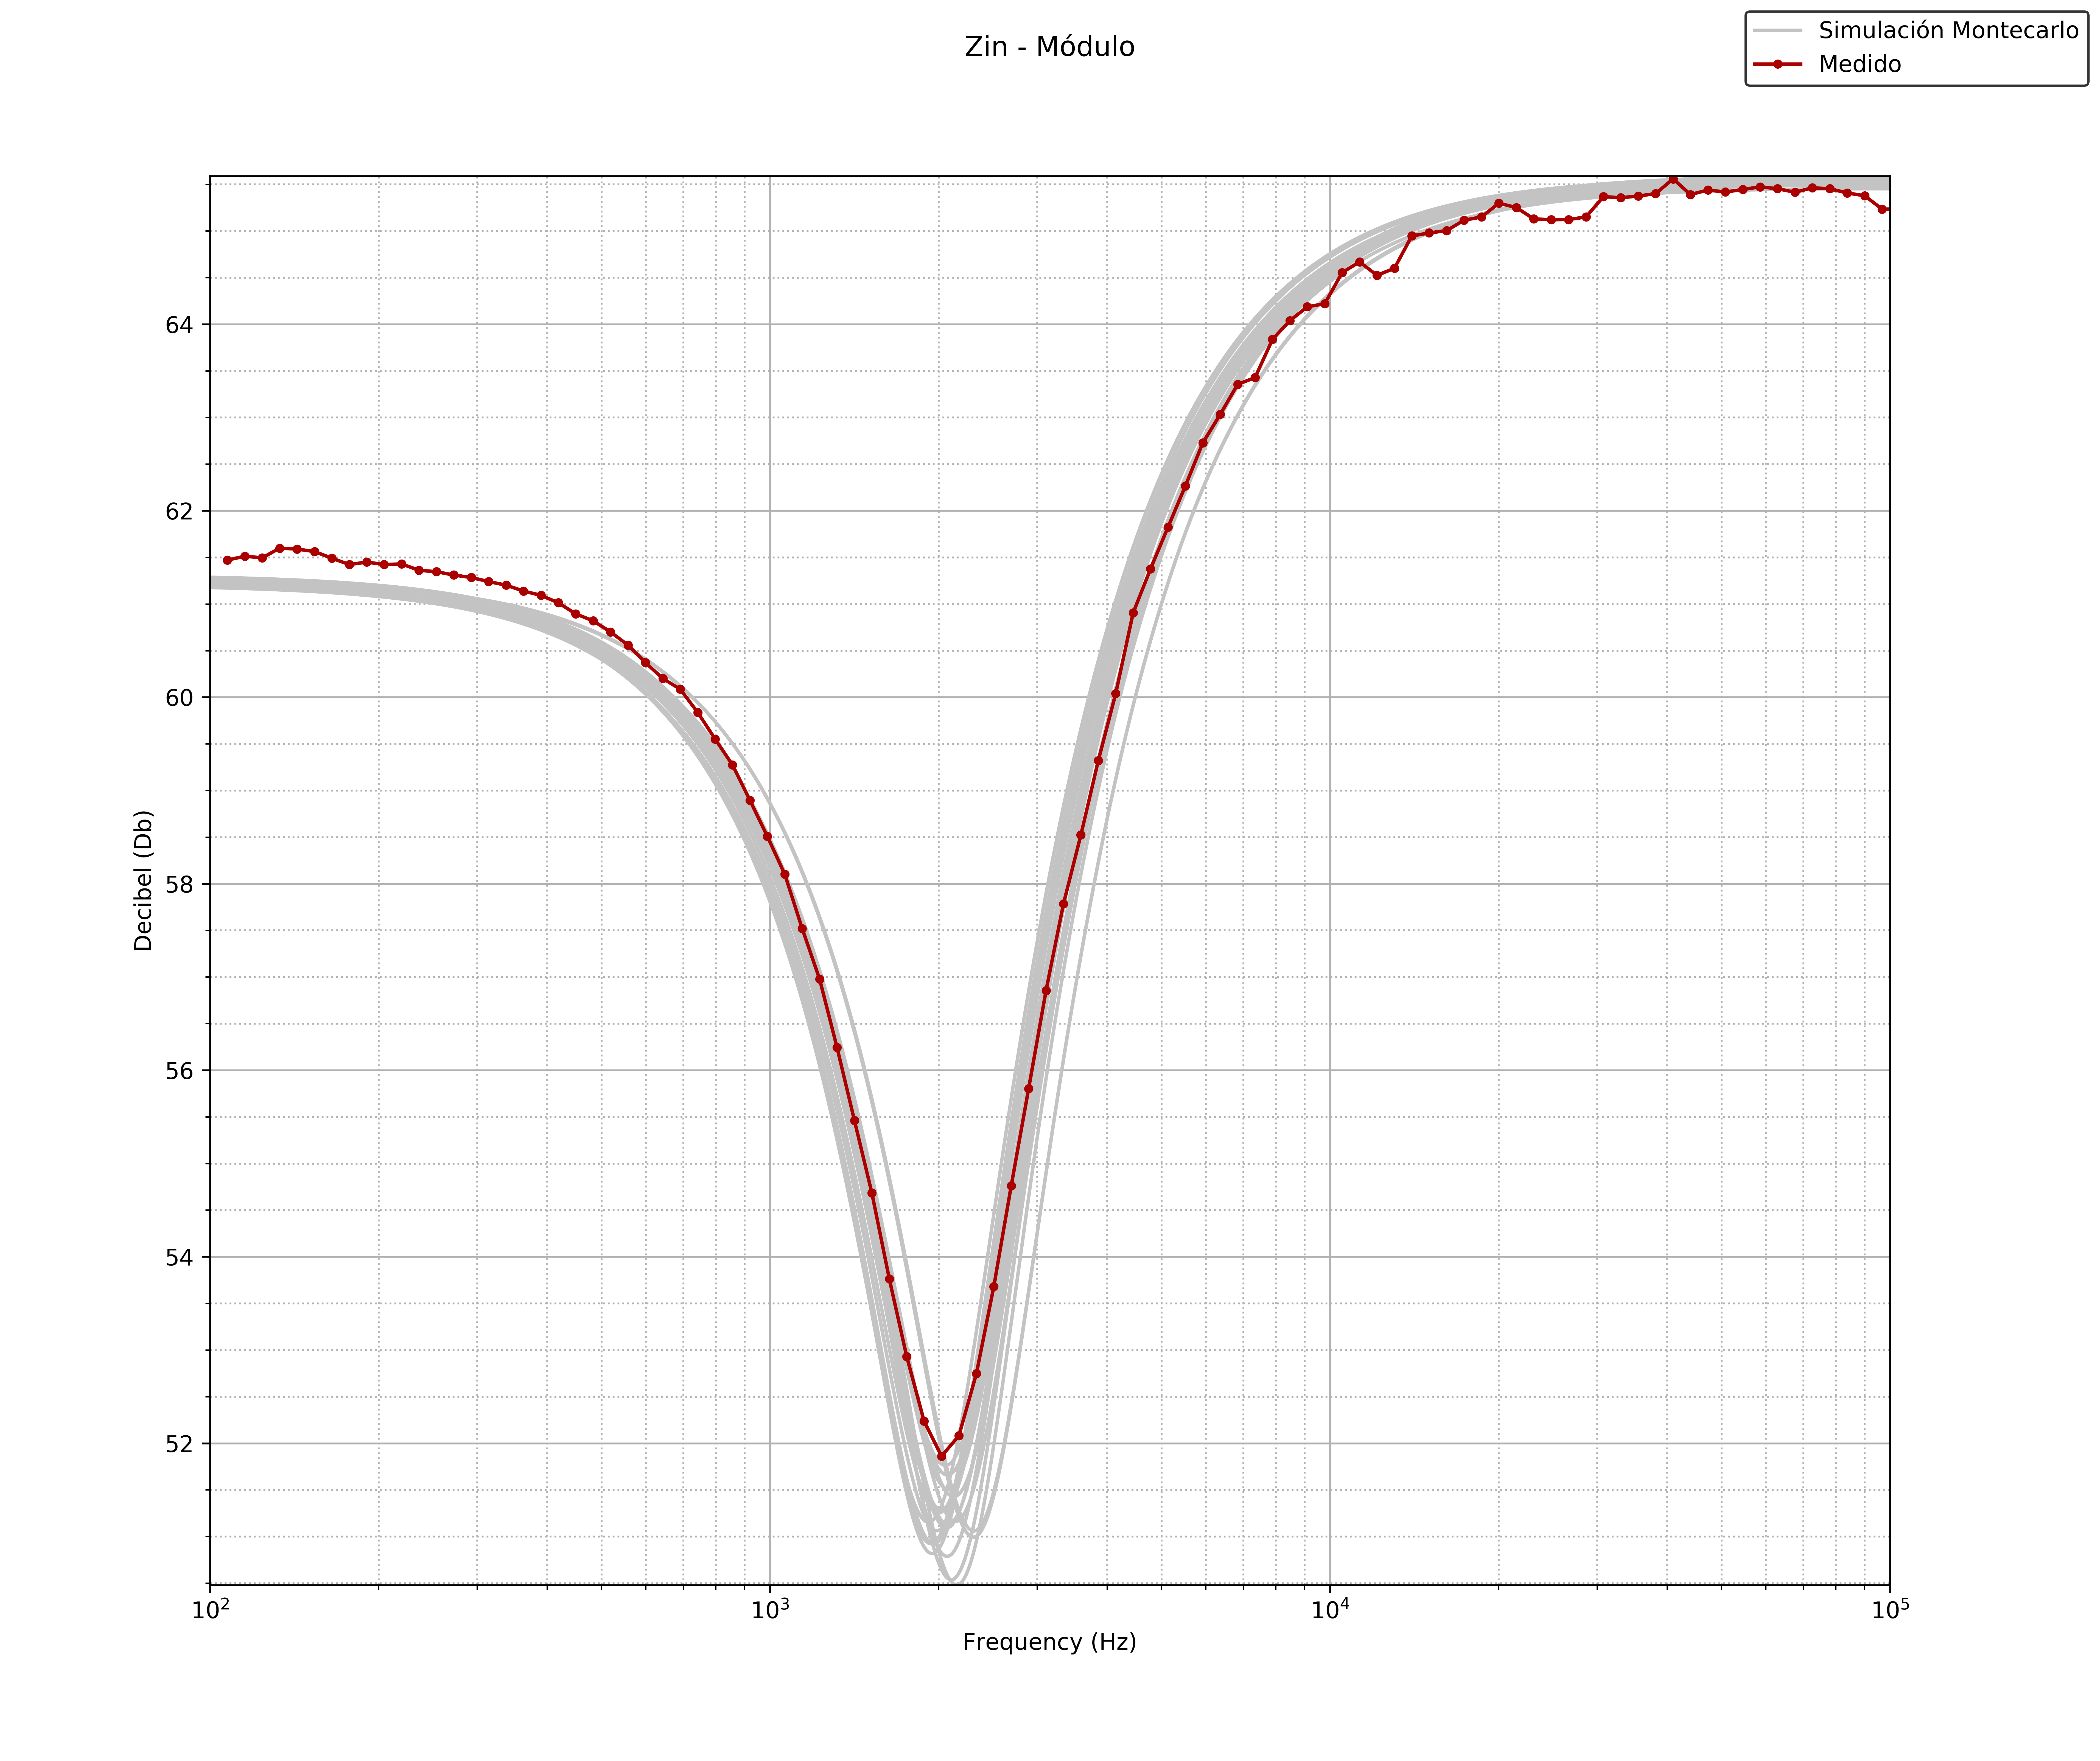
\includegraphics[width=10cm,height=10cm,keepaspectratio]{../EJ1/00GRAFICOS/zin_modulo_sinTeorico.png}
	\caption{Impedancia de entrada.}
	\label{zin_mod}
\end{figure}

\subsection{Impedancia de salida}

En esta parte se detallar\'a el m\'etodo empleado para medir la impedancia de salida, pero se anticipa al lector que no se considera que el mismo haya funcionado como se esperaba. 

Al tener un circuito con componentes activos, desde un primer momento se descart\'o la opci\'on de medir la impedancia de salida pasivando la fuente de entrada y colocando una fuente a la salida para medirla como si esta fuera una impedancia de entrada vista desde la nueva fuente. Por esta raz\'on se prosigui\'o de la siguiente forma.

\begin{figure}[H] %!ht
	\centering
	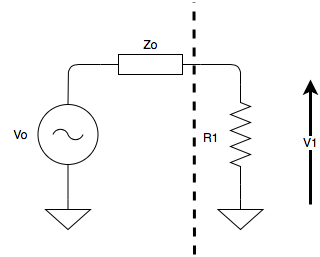
\includegraphics[width=8cm,height=8cm,keepaspectratio]{../EJ1/00GRAFICOS/zout.png}
	\caption{Impedancia de entrada.}
	\label{zout}
\end{figure}

El circuito de la figura \ref{zout} representa a nuestro circuito en el momento de medir. Se considera como circuito equivalente para el high pass notch a una fuente de tensi\'on $Vo$ en serie con la $Zo$ que se quiere medir. Primero se conecta a la salida del circuito una resistencia R1 y se mide la tensi\'on $V1$ sobre sus bornes. Luego se hace lo mismo con una resistencia R2, y se mide la tensi\'on sobre sus bornes, $V2$. Por divisor resistivo de tensi\'on:

\begin{equation}
\begin{cases}
	V_1 = \frac{Vo R_1}{Zo + R_1}\\
	V_2 = \frac{Vo R_2}{Zo + R_2}
\end{cases}
\label{v1v2}
\end{equation}

Considerando la misma $Vo$ para ambos casos, se dividen ambas expresiones de forma que se cancele dicha tensi\'on y se obtenga:

\begin{equation}
\frac{V_1}{V_2} = \frac{R_1}{Zo + R_1 } \cdot \frac{Zo + R_2}{R_2}
\end{equation}

Luego llamando $K = \frac{V_1}{V_2}\cdot \frac{R_2}{R_1} = \frac{Zo + R_2}{Zo + R_1}$, se obtiene:

\begin{equation}
\begin{cases}
Zo = \frac{R_2 - R_1 \cdot K}{K - 1}\\
K=\frac{V_1 R_2}{V_2 R_1}
\end{cases}
\label{zo}
\end{equation}

Para este m\'etodo, las resistencias empleadas a la salida deb\'ian ser, en nuestro caso, del orden de los $k\Omega$, para evitar que se rompiera la realimentaci\'on del opamp de salida, debido a la corriente. Se usaron resistencias de $33k\Omega$, $2k7\Omega$ y $10k\Omega$ con la finalidad de chequear el valor luego obtenido de la Zo a partir de m\'as de un par de resistencias, para disminuir la posibilidad de error.
Previamente se simularon las tensiones de salida con las mismas resistencias y considerando las puntas del osciloscopio y se observ\'o que daban igual. Esto implicar\'ia que al momento de medir no podr\'ia haber mucha diferencia de tensi\'on a la salida y dificultar\'ia el m\'etodo. Y as\'i fue. Se obtuvo una diferencia de tensi\'on de salida entre los distintos casos del orden de los $mV$, de forma que para calcular la Zo esa diferencia de tensi\'on estar\'ia en el nivel del piso de ruido. Realizar operaciones matem\'aticas sobre esta diferencia de tensi\'on tan chica, no ser\'ia un m\'etodo confiable.

\begin{figure}[H] %!ht
	\centering
	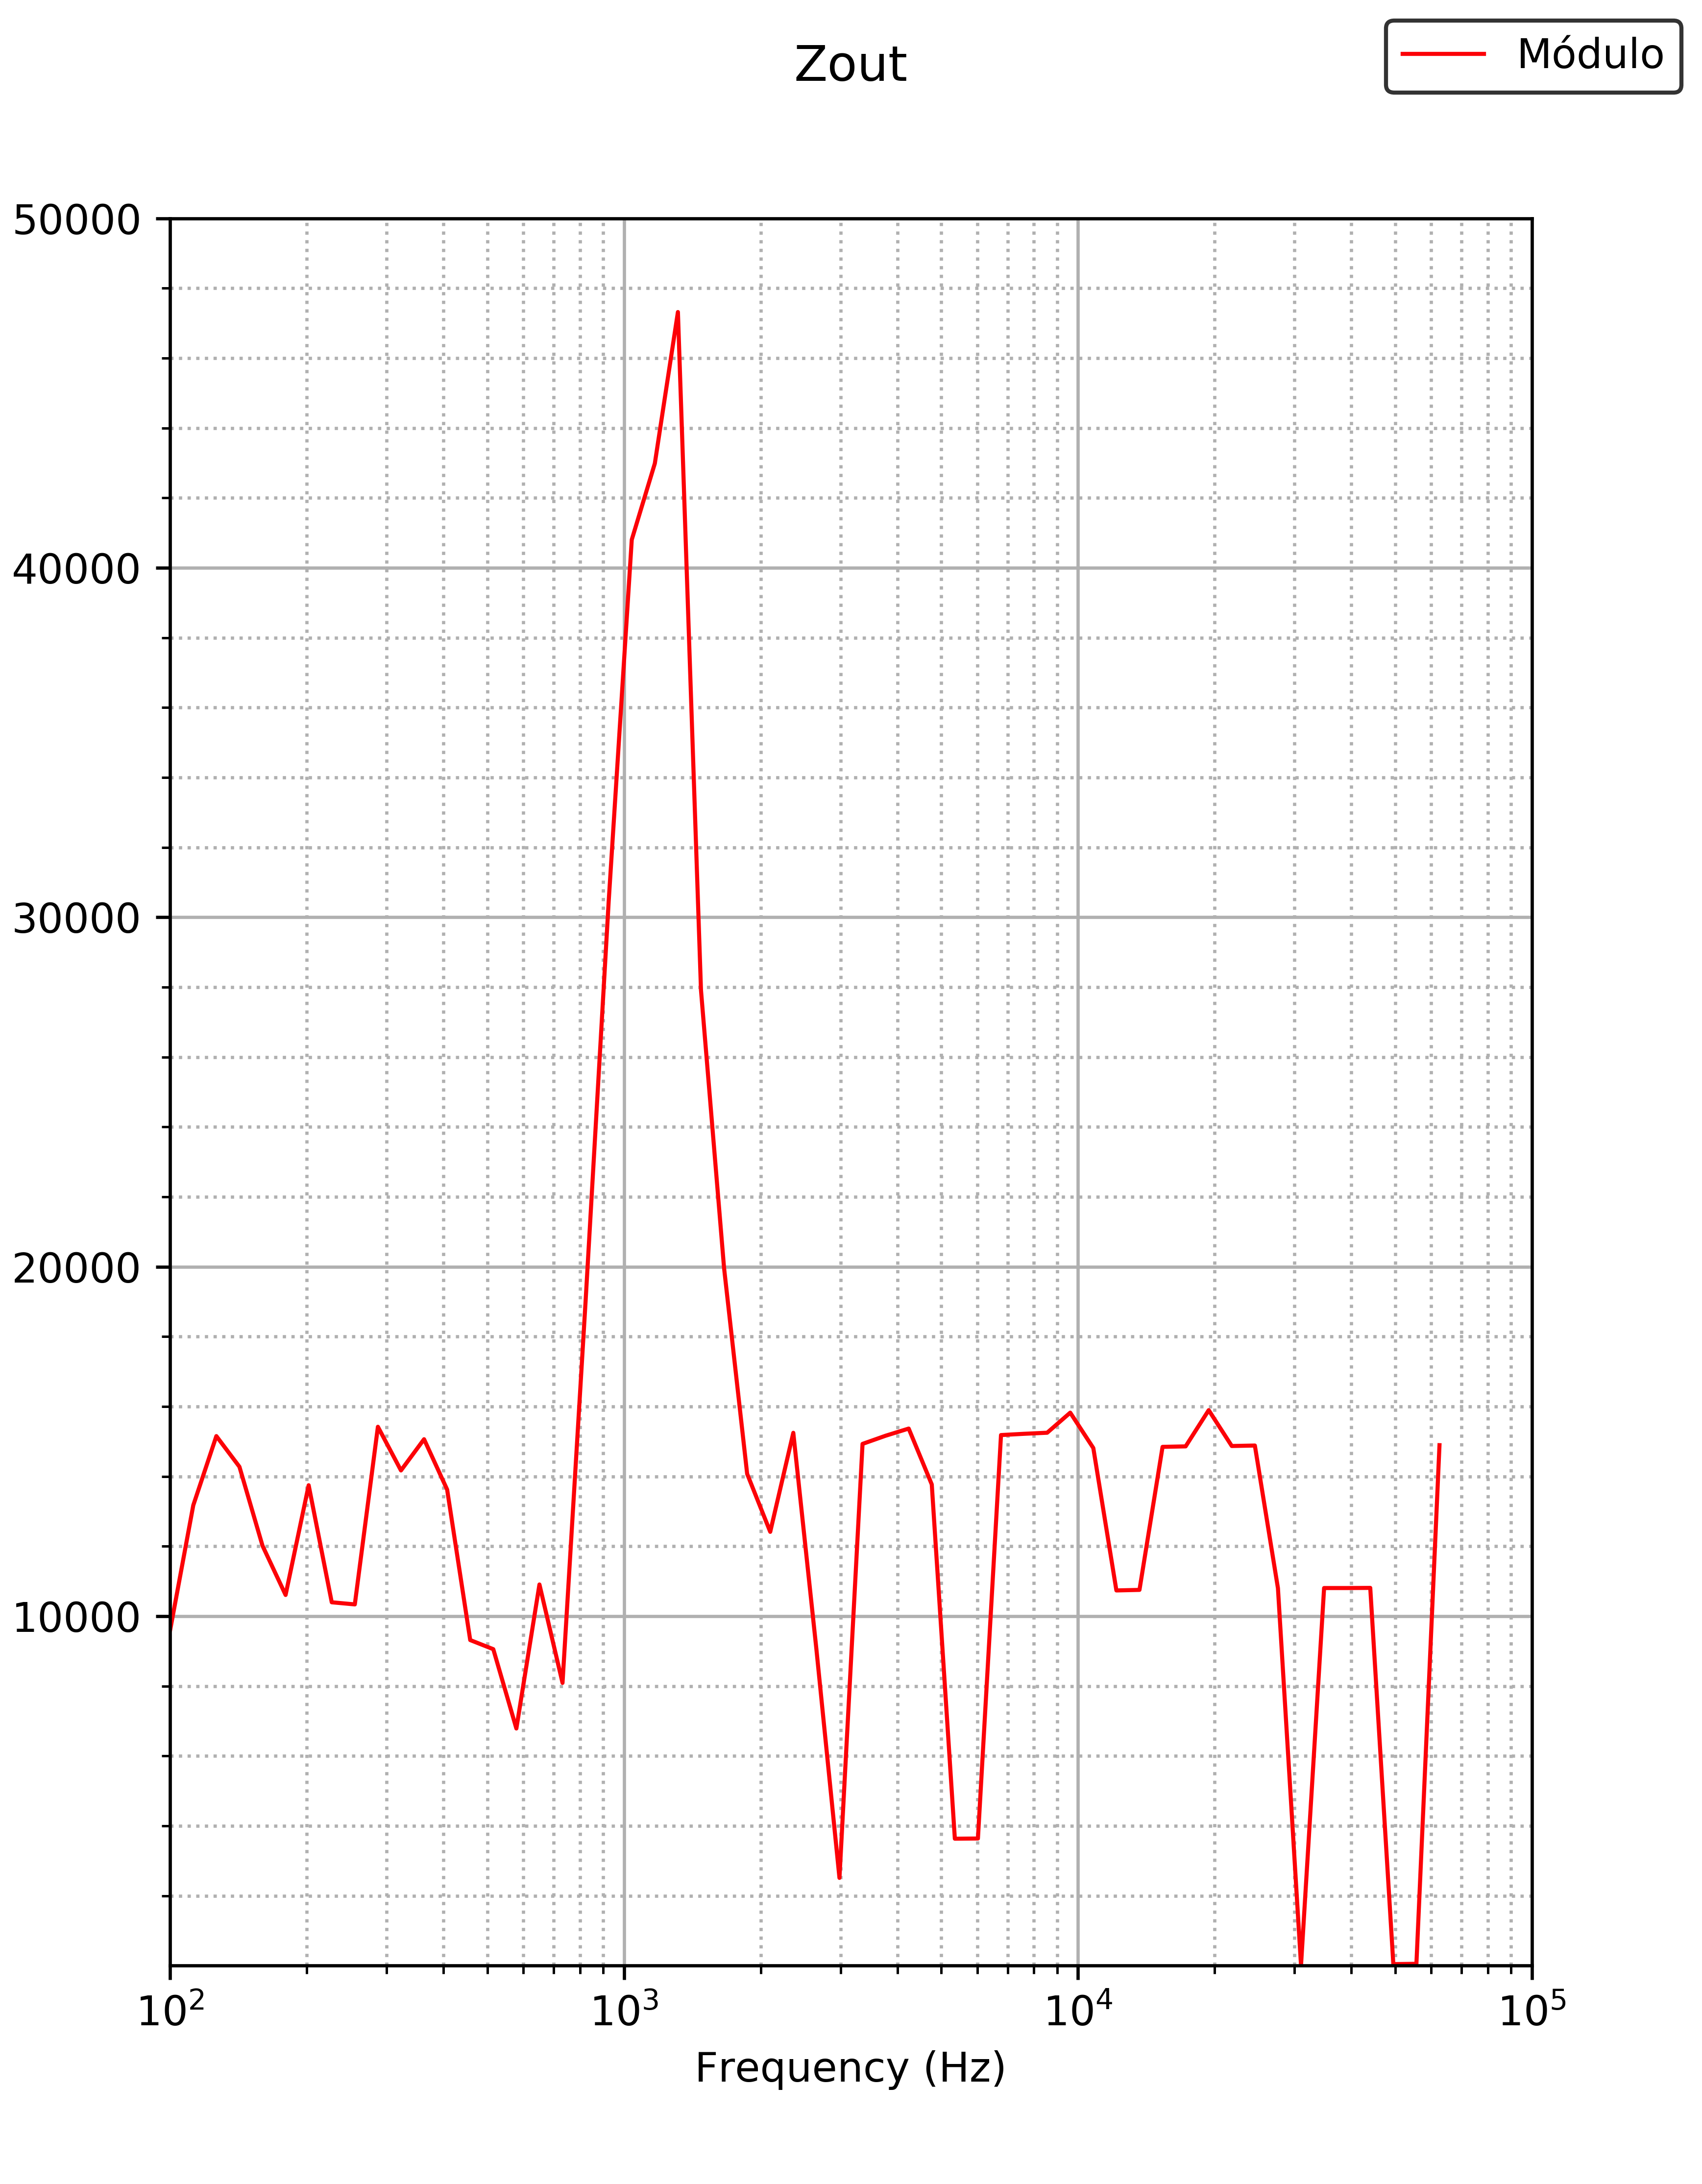
\includegraphics[width=10cm,height=10cm,keepaspectratio]{../EJ1/00GRAFICOS/zom.png}
	\caption{"Impedancia de salida" medida.}
	\label{zom}
\end{figure}

Algo interesante que se observa en el gr\'afico \ref{zom} es que hay un pico en su amplitud en la zona de frecuencias donde se encuentra el pico del filtro Notch. Sin embargo, no podemos afirmar que est\'e bien o mal lo obtenido. El gr\'afico fue logrado mediante c\'alculos con n\'umeros complejos para poder obtener Zo, pero las simulaciones, al haber sido tambi\'en sobre las tensiones medidas, requerir\'ian pasar por los mismos c\'alculos, lo cual impide que de forma r\'apida se sepa si est\'a bien lo obtenido (m\'as all\'a de la limitaci'on previamente mencionada sobre la gran probabilidad de tener error en el resultado al tener una diferencia de tensi\'on en el orden del piso de ruido).


